\documentclass[a4paper,12pt]{article} % тип документа

% Поля страниц
\usepackage[left=2.5cm,right=2.5cm,
    top=2cm,bottom=2cm,bindingoffset=0cm]{geometry}
    
%Пакет дял таблиц   
\usepackage{multirow} 
    
%Отступ после заголовка    
\usepackage{indentfirst}


% Рисунки
\usepackage{floatrow,graphicx,calc}
\usepackage{wrapfig}

%%% Работа с картинками
\usepackage{graphicx}  % Для вставки рисунков
\graphicspath{{images/}{images2/}}  % папки с картинками
\setlength\fboxsep{3pt} % Отступ рамки \fbox{} от рисунка
\setlength\fboxrule{1pt} % Толщина линий рамки \fbox{}
\usepackage{wrapfig} % Обтекание рисунков и таблиц текстом

% Создаёем новый разделитель
\DeclareFloatSeparators{mysep}{\hspace{1cm}}

% Ссылки?
\usepackage{hyperref}
\usepackage[rgb]{xcolor}
\hypersetup{				% Гиперссылки
    colorlinks=true,       	% false: ссылки в рамках
	urlcolor=blue          % на URL
}


%  Русский язык
\usepackage[T2A]{fontenc}			% кодировка
\usepackage[utf8]{inputenc}			% кодировка исходного текста
\usepackage[english,russian]{babel}	% локализация и переносы




% Математика
\usepackage{amsmath,amsfonts,amssymb,amsthm,mathtools}

%%% Дополнительная работа с математикой
\usepackage{amsmath,amsfonts,amssymb,amsthm,mathtools} % AMS
\usepackage{icomma} % "Умная" запятая: $0,2$ --- число, $0, 2$ --- перечисление


% Что-то 
\usepackage{wasysym}


\begin{document}
\begin{center}
	\footnotesize{МОСКОВСКИЙ ФИЗИКО-ТЕХНИЧЕСКИЙ ИНСТИТУТ\\(НАЦИОНАЛЬНЫЙ 			ИССЛЕДОВАТЕЛЬСКИЙ УНИВЕРСИТЕТ)}\\
	\footnotesize{ФИЗТЕХ-ШКОЛА РАДИОТЕХНИКИ И КОМПЬЮТЕРНЫХ ТЕХНОЛОГИЙ\\}
	\hfill \break
	\hfill \break
	\hfill \break
	\hfill \break
	\hfill \break
	\hfill \break
\end{center}

\begin{center}   
    \hfill \break
	\hfill \break
	\hfill \break
	\hfill \break
	\hfill \break
	\hfill \break
	\hfill \break
	\hfill \break
	\hfill \break
	\hfill \break
	\hfill \break
	\large{Лабораторная работа № 3.2.2\\\large{\textbf{Резонанс напряжений в последовательном контуре}}}\\
	\hfill \break
	\hfill \break
	\hfill \break
	\hfill \break
	\hfill \break
	\hfill \break
	\hfill \break
	\hfill \break
	\hfill \break
	\hfill \break
	\hfill \break
	\begin{flushright}
		Климова Екатерина\\
		Группа Б01-108
	\end{flushright}
	\hfill \break
\end{center}
\hfill \break
\hfill \break
\begin{center}
	Долгопрудный, 2022 г.
\end{center}
\thispagestyle{empty}

\newpage
\hfill \break
\textbf{Цель работы:} исследование резонанса напряжений в последовательном колебательном контуре с изменяемой емкостью, получение амплитудно- и фазово-частотных характеристик, определение основных параметров контура.
\hfill \break
\hfill \break
\textbf{В работе используются:} генератор сигналов; источник напряжения, нагрузкой которого явлется последовательный колебательный контур с переменной емкостью; двухканальный осциллограф; цифровые вольтметры.

\section{Аннотация}
\hfill \break В данной работе проводится исследование колебаний напряжения в последовательном колебательном контуре под воздействием внешней синусоидальной ЭДС. Проводится получение АЧХ и ФЧХ контура, при помощи которых определяются добротность и другие характеристики колебательного контура.

\section{Теоретические сведения}
\subsection{Вынужденные колебания}
\hfill \break Рассмотрим процессы, протекающие в $RLC$-контуре, подключенном к источнику внешней ЭДС, изменяющейся по гармоническому закону $\varepsilon = \varepsilon_{0}\cos{(\omega t + \varphi_{0})}$. Тогда для напряжения в конденсаторе получим уравнение:

\begin{equation}\label{ linkname }
\ddot{U_{c}} + 2\gamma \dot{U_{c}} + \omega_{0}^2U_{c} = \omega_{0}^2\varepsilon_{0}\cos{(\omega t + \varphi_{0})},
\end{equation}

\begin{wrapfigure}{l}{0.2\textwidth}
\begin{center}
    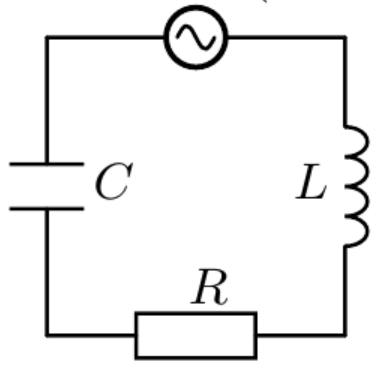
\includegraphics[width=1\textwidth]{3.2.2_1.png}
    \textbf{Рис. 1.} Последовательный контур с внешней ЭДС
\end{center}
\end{wrapfigure}

\hfill \break решение которого будет состоять из общего решения однородного дифференциального уравнения и какого-либо частного решения данного уравнения с правой частью. Для нахождения этого частного решения воспользуемся \textbf{методом комплексных амплитуд}. То есть \textit{пусть некоторая комплексная функция $f(t)$ является решением линейного дифференциального уравнения с вещественными коэффициентами и комплексной правой частью; тогда вещественная часть этой функции $Re f(t)$ является решением того же уравнения, в правой части которого стоит вещественная часть прежнего выражения, а мнимая часть $Im f(t)$ $-$ решением уравнения с мнимой правой частью.} Тогда уравнение (1) станет выглядеть так:

\begin{equation}\label{ linkname }
\ddot{U_{c}} + 2\gamma \dot{U_{c}} + \omega_{0}^2U_{c} = \omega_{0}^2\varepsilon,
\end{equation}

\hfill \break где $\varepsilon_{0}e^{i\varphi}$ называется \textbf{комплексной амплитудой}. 

\hfill \break Решив уравнение (2), получим комплексное выражение для напряжения на конденсаторе, вещественная часть которого и является решением исходного уравнения. Комплексные амплитуды тока в контуре и напряжений на сопротивлении и индуктивности:

\begin{equation}\label{ linkname }
\textbf{U}_{C0} = \frac{\varepsilon_{0}}{i\omega CZ}, \text{       } Z = R + i(\omega L - \frac{1}{\omega C}),
\end{equation}

\begin{equation}\label{ linkname }
\textbf{I}_{0} = \frac{\varepsilon_{0}}{Z}, \text{                 } \textbf{U}_{R0} = \frac{R\varepsilon_{0}}{Z}, \text{                    } \textbf{U}_{L0} = i\omega L\frac{\varepsilon_{0}}{Z}.
\end{equation}

\hfill \break Определим величину $Z$ $-$ \textbf{импеданс}, или комплексное сопротивление, $-$ характеристику колебательного контура на заданной частоте:

$$
Z_{R} = R, \text{ } Z_{L} = i\omega L, \text{ } Z_{C} =  \frac{1}{i\omega C}.
$$

\hfill \break \textit{Активным} сопротивлением называется действительная часть $Z$, \textit{реактивным} $-$ мнимая: $Im Z = \omega L - \frac{1}{\omega C}$. Импедансы реальных конеднсаторов и катушек содержат, кроме мнимой части, также и действительную часть. Действительная часть импеданса определяется необратимыми потерями энергии, которые могут быть связаны как с омическим сопротивлением проводников, так и с другими причинами: с утечками и диэлектрическими потерями в конденсаторах, с токами перемагничивания в катушках. Потери в катушках самоиндукции и конденсаторах зависят как от частоты, так и от амплитуды проходящего через них тока. Импедансы контура и его отдельных элементов могут быть представлены в показательной форме:

\begin{equation}\label{ linkname }
Z = Z_{0}e^{i\psi},
\end{equation}

\hfill \break где $Z_{0}$ $-$ модуль комплексного числа, $\psi = arg Z$ $-$ его аргумент. Для импеданса рассматриваемого последовательного контура находим:

\begin{equation}\label{ linkname }
Z_{0} = \sqrt{(Re Z)^2 + (Im Z)^2} = \frac{R}{\cos{\psi_{I}}},
\end{equation}

\begin{equation}\label{ linkname }
\tg{\psi_{I}} = \frac{Im Z}{Re Z} = \frac{\omega L - \frac{1}{\omega C}}{R}.
\end{equation}

\hfill \break Так, действительная часть тока в контуре:

\begin{equation}\label{ linkname }
I(t) = \frac{\varepsilon_{0}}{R} \cos{\psi_{I}} \cos({\omega t + \varphi_{0} - \psi_{I}}).
\end{equation}

\hfill \break Как видно из (8), угол $\psi_{I}$, определяемый отношением мнимой и действительной частей импеданса, представляет собой сдвиг фаз между напряжением на последовательном контуре и током в нем, причем положительные значения этого угла соответствуют отставанию фазы тока, а отрицательные $-$ опережению. В общем случае, когда к источнику последовательно подключены резистор, конденсатор и катушка, сдвиг фазы тока лежит в пределах $-\pi/2 < \psi_{I} < \pi/2$. От этого угла также зависит амплитуда силы тока.

\subsection{Векторные диаграммы}
\hfill \break Решения, полученные методом комплексных амплитуд, допускают простую геометрическую интерпретацию. Комплексное число, например, напряжение $\varepsilon =\varepsilon_{0}e^{i(\omega t + \varphi_{0})}$, представляется на комплексной плоскости вектором, длина которого равна $\varepsilon_{0}$, а угол, составляемый этим вектором с  вещественной осью, равен $(\omega t + \varphi_{0})$ $-$ фазе напряжения. Вектор напряжения вращается со скоростью $\omega$ против часовой стрелки. Удобно перейти к системе координат, которая сама вращается с такой угловой скоростью. В этой системе вектор $\varepsilon$ будет представлен покоящимся вектором $\varepsilon_{0}e^{i \varphi}$, а векторы $\textbf{I}_{0}$, $\textbf{U}_{C0}$, $\textbf{U}_{L0}$, $\textbf{U}_{R0}$ тоже будут неподвижны, но окажутся сдвинутыми по углу относительно вектора $\varphi_{0}$. Вектор $\textbf{I}_{0}$, как показано выше, сдвинут от вектора $\varphi_{0}$ на угол $\psi_{I}$. Построенная таким образом диаграмма называется \textit{векторной}.

\subsection{Резонанс напряжений в последовательном контуре}
\hfill \break Запишем вещественные части решений уравнений (3)-(4):

\begin{equation}\label{ linkname }
I(t) = \frac{U_{R}(t)}{R} = I_{\omega}\cos{(\omega t - \psi_{I})}, \text{ } I_{\omega} = \frac{\varepsilon_{0}}{Z_{0}},
\end{equation}

\begin{equation}\label{ linkname }
Z_{0} = R\sqrt{1 + [\frac{\rho}{R}(\frac{\omega}{\omega_{0}} - \frac{\omega_{0}}{\omega})]^2}, \text{ } \psi_{I} = \arctg{[\frac{\rho}{R}(\frac{\omega}{\omega_{0}} - \frac{\omega_{0}}{\omega})]},
\end{equation}

\begin{equation}\label{ linkname }
U_{C}(t) = U_{C\omega}\cos{(\omega t - \psi_{C})}, \text{ } U_{C\omega} = \varepsilon_{0}\frac{\rho}{Z_{0}}\frac{\omega_{0}}{\omega}, \text{ } \psi_{C} = \psi_{I} + \pi/2,
\end{equation}

\begin{equation}\label{ linkname }
U_{L}(t) = U_{L\omega}\cos{(\omega t - \psi_{L})}, \text{ } U_{L\omega} = \varepsilon_{0}\frac{\rho}{Z_{0}}\frac{\omega}{\omega_{0}}, \text{ } \psi_{L} = \psi_{I} - \pi/2.
\end{equation}

\hfill \break Анализ полученных формул (9)-(12) позволяет сделать следующие выводы:
\begin{enumerate}
\item{При заданных параметрах $\varepsilon_{0}$ и $\omega_0$ внешнего источника напряжения зависимости амплитуд и фаз тока и напряжений в системе от частоты $-$ амплитудные и частотные характеристики $-$ определяются двумя безразмерными величинами $\rho/R$ и $\omega/\omega_{0}$. Для контура со слабым затуханием ($Q \gg 1$) имеет место соотношение $Q \approx \frac{\rho}{R}$.}
\item{Поведение системы носит резонансный характер: при $\omega = \omega_{0}$, когда мнимая часть импеданса равна нулю и $\omega_{0} L = \frac{1}{\omega_{0}C} = \rho, \text{ } Im Z = 0, \text{ } Z_{0} = R, \text{ } \psi_{I} = 0$ амплитуды тока и напряжения на сопротивлении достигают максимальных значений ($I_{\omega_0} = \varepsilon_{0}/R, \text{ } U_{R\omega_0} = \varepsilon_{0}$) и совпадают по фазе с ЭДС. Таким образом, последовательный контур на собственной частоте $\omega_{0}$ представляет для внешней ЭДС чисто активную нагрузку, на которой выделяется мощность $P_\text{max} = \varepsilon_{0}^2/2R$.
\item{Наиболее ярко резонансный характер проявляется в напряжениях на конденсаторе и индуктивности, которые при $\omega = \omega_{0}$ в $\rho/R$ раз превышают напряжение $\varepsilon_{0}$ по амплитуде и сдвинуты по фазе от него каждый на $\pi/2$, то есть находятся в противофазе друг с другом. При высокой добротности их амплитуды значительно превышают амплитуду напряжения на контуре. По этой причине резонанс в последовательном контуре называется \textit{резонансом напряжений}.}
\end{enumerate}

\begin{equation}\label{ linkname }
U_{C\omega}^{\text{рез}} = U_{L\omega}^{\text{рез}} = \frac{\rho}{R}\varepsilon_{0}\left( 1-\frac{\rho^2}{4R^2} \right) ^{-1/2}.
\end{equation}

\hfill \break Частоты, на которых достигаются максимальные значения величин, характеризующих вынужденные колебания в различных колебательных системах, принято называть резонансными. Для напряжения на конденсаторе резонансной является частота

\begin{equation}\label{ linkname }
\omega_{C}^{\text{рез}} = \omega_{0} \left( 1-\frac{\rho^2}{2R^2} \right) ^{+1/2},
\end{equation}

\hfill \break для напряжения на индуктивности $-$

\begin{equation}\label{ linkname }
\omega_{L}^{\text{рез}} = \omega_{0} \left( 1-\frac{\rho^2}{2R^2} \right) ^{-1/2},
\end{equation}

\hfill \break причем $\omega_{C}^{\text{рез}} \cdot \omega_{L}^{\text{рез}} = \omega_{0}^2$. 

\hfill \break На рис. 2 приведены в безразмерном виде кривые зависимостей от $x = \omega/\omega_{0}$ амплитуды тока (а) $j(x) = RI_{\omega}/\varepsilon_{0}$ и амплитуды напряжения на конденсаторе (б) $u(x) = U_{C\omega}/\varepsilon_{0}$. Эти кривые называются амплитудными резонансными кривыми последовательного колебательного контура. Важными характеристиками резонансных кривых являются максимальное значение амплитуды соответствующей величины и \textit{ширина резонансной кривой}, при которой аплитуда уменьшается в $\sqrt{2}$ раз по сравнению со своим максимальным значением (мощность сигнала уменьшается в два раза). В частности, по этим кривым можно определить добротность колебательного контура:

\begin{equation}\label{ linkname }
Q = \frac{U_{C}^{\text{рез}}}{\varepsilon_{0}}.
\end{equation}

\begin{center}
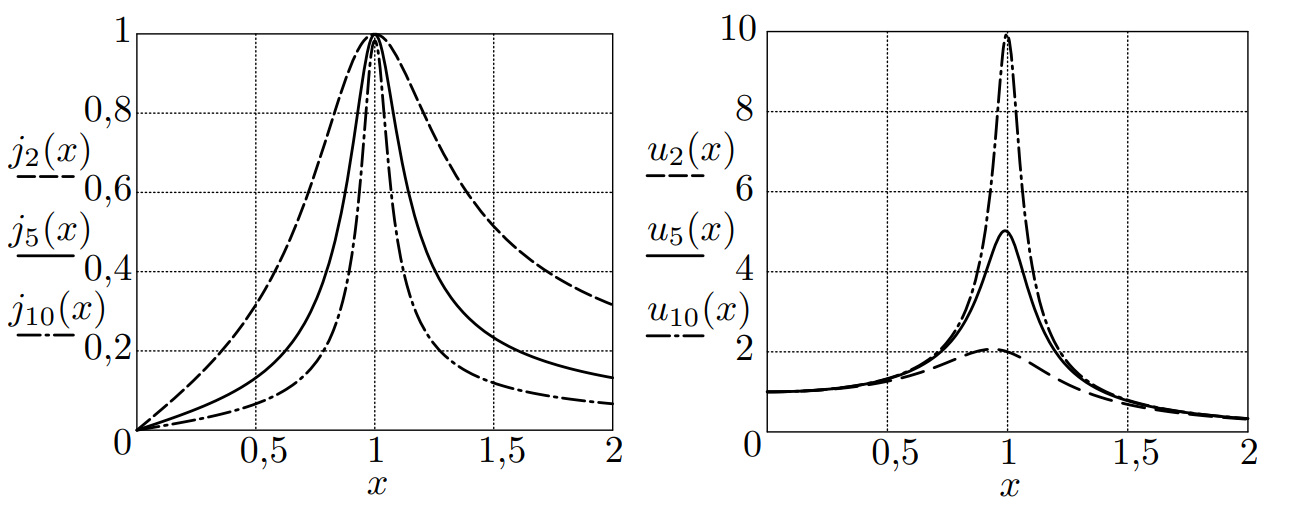
\includegraphics[width=0.85\textwidth]{3.2.2_2.png}\\
\textbf{Рис. 2.}  Амплитудные резонансные кривые а) тока и б) напряжения последовательного колебательного контура в безразмерных переменных ($x = \omega/\omega_{0}$) при $\rho/R =$ 2, 5 и 10\\ 
\end{center}

\hfill \break Наибольший практический интерес представляет случай, когда отклонение $\Delta \omega = \omega - \omega_{0}$ частоты внешней ЭДС от собственной частоты контуры с добротностью $Q = \rho/R \gg 1$ удовлетворяет сильному неравенству $|\Delta \omega| \ll \omega_{0}$. При этом в первом порядке малости по относительной расстройке частоты $\Delta \omega/\omega_{0}$

$$
\frac{\omega}{\omega_{0}} - \frac{\omega_{0}}{\omega} = \frac{2\Delta\omega}{\omega_{0}},
$$

\hfill \break откуда

$$
Z_{0} = R\sqrt{1+(\tau\Delta\omega)^2}, \text{ } \psi_{I} = \arctg{\tau\Delta\omega},
$$

\hfill \break где $\tau = 1/\gamma$ $-$ время затухания колебательного контура. В резонансе, когда для высокодобротного контура $\omega = \omega_{0}$, $\Delta \omega = 0$, выражения для амплитуд тока и напряжений на емкости и индуктивности, фазовых сдвигов принимают вид:

\begin{equation}\label{ linkname }
I_{\omega}(\omega_{0}) = \frac{\varepsilon_{0}}{R}, \text{ } \psi_{I} (\omega_{0}) = 0,
\end{equation}
\begin{equation}\label{ linkname }
U_{C\omega} (\omega_{0}) = Q\varepsilon_{0}, \text{ } \psi_{C} (\omega_{0}) = \frac{\pi}{2},
\end{equation}
\begin{equation}\label{ linkname }
U_{L\omega} (\omega_{0}) = Q\varepsilon_{0}, \text{ } \psi_{L} (\omega_{0})  = -\frac{\pi}{2}.
\end{equation}

\hfill \break Величина $\delta \omega = 2|\Delta \omega_{\gamma}| = 2\gamma = 2/\tau$ представляет собой \textit{ширину резонансной кривой} $U_{C} (\omega)$, по которой с учетом соотношений $Q = \omega_{0}/2\gamma = \tau\omega_{0}/2$, зная $\omega_{0}$, можно найти добротность контура

\begin{equation}\label{ linkname }
Q = \frac{\omega_{0}}{\delta\omega}.
\end{equation}

\section{Экспериментальная установка}

\hfill \break Схема экспериментальной установки показана на рис. 3. Синусоидальный сигнал от генератора поступает на вход управляемого напряжением источника напряжения, собранного на операционном усилителе, питание которого осуществляется встроенным блоком-выпрямителем от сети. Источник напряжения (источник с нулевым внутренним сопротивлением) обеспечивает с высокой точностью постоянство амплитуды сигнала $\varepsilon = \varepsilon_{0}\cos{(\omega t + \varphi_{0})}$ на меняющейся по величине нагрузке $-$ последовательном колебательном контуре, изображенном на рис. 3 в виде эквивалентной схемы. 

\begin{center}
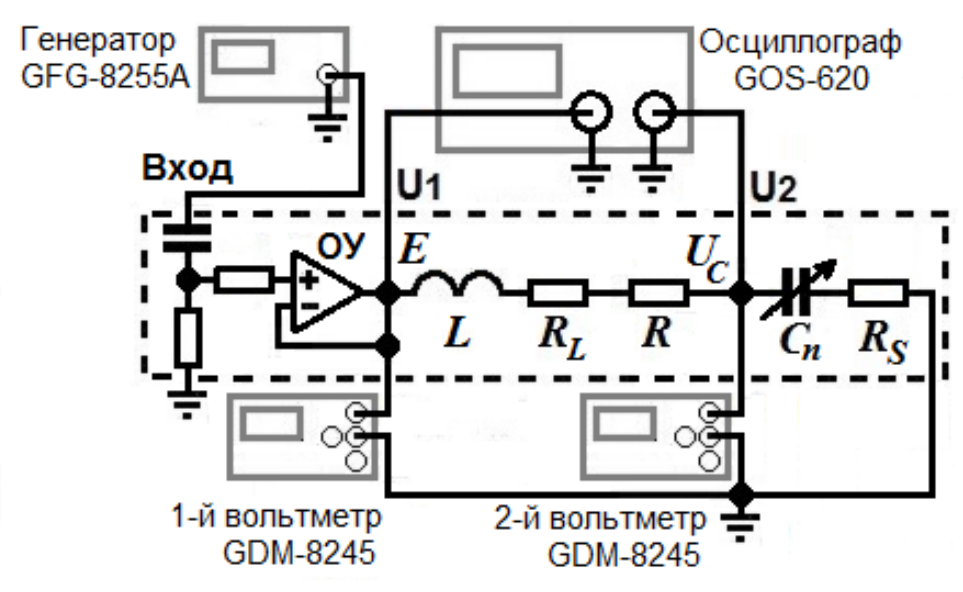
\includegraphics[width=0.75\textwidth]{3.2.2_3.png}\\
\textbf{Рис. 3.}  Схема экспериментальной установки\\ 
\end{center}

\hfill \break Источник напряжения, колебательный контур и блок питания заключены в отдельный корпус, отмеченный на рисунке штриховой линией. На корпусе имеются коаксиальные разъемы <<Вход>>, <<$U_{1}$>>, <<$U_{2}$>>, а также переключатель магазина емкостей $C_{n}$ с указателем номера $n$. Напряжение $E$ на контуре через разъем <<$U_{1}$>> попадает одновременно на канал 1 осциллографа и вход 1-го цифрового вольтметра. Напряжение на конденсаторе $U_{C}$ подается через разъем <<$U_{2}$>> одновременно на канал 2 осциллографа и вход 2-го цифрового вольтметра.

\hfill \break В нашем контуре катушка индуктивности обладает малым сопротивлением по постоянному току и высокой собственной резонансной частотой $f_{r} > 1.3$ МГц. В общем случае каждая катушка, помимо индуктивности, характеризуется также собственной (межвитковой) емкостью $C_{L}$ и активным сопротивлением потерь $R_{L}$. Считается, что эти величины сосредоточены в отдельных элементах схемы, образующих с $L$ замкнутую колебательную цепь с собственной резонансной частотой $f_{r} = 1/2\pi \sqrt{LC_{L}}$. Вследствие влияния емкости $C_{L}$ при измерении на частоте $f$ определяется не истинная индуктивность $L$, а ее эффективное значение $L_\text{эфф} = L/(1-f^2/f_{r}^2)$, однако в нашей работе $f \ll f_{r}$, так что индуктивность представлена своим истинным значением.

\hfill \break Для оценки возможного вклада активных потерь в конденсаторах в общий импеданс контура воспользуемся представлением конденсатора с емкостью $C$ последовательной эквивалентной схемой на рис. 4:

\begin{center}
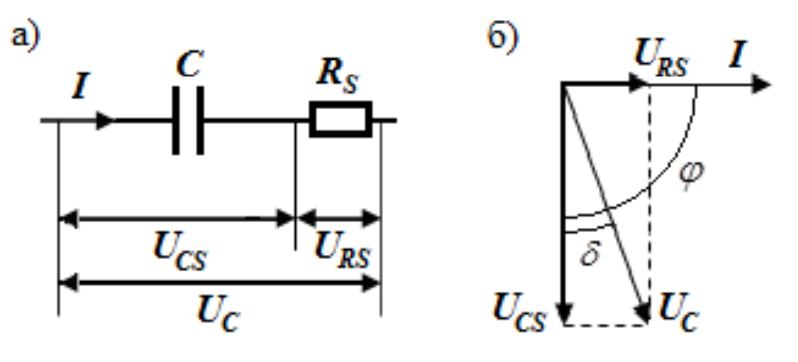
\includegraphics[width=0.55\textwidth]{3.2.2_4.png}\\
\textbf{Рис. 4.}  Последовательная эквивалентная схема для конденсатора с потерями\\ 
\end{center}

\hfill \break На этой схеме $R_{s}$ $-$ это так называемое эквивалентное последовательное сопротивление (ЭПС), обусловленное электрическим сопротивлением материала обкладок и выводов конденсатора и контактов между ними, а также потерями в диэлектрике. Из векторной диаграммы (рис. 4б) видно, что активные потери в конденсаторе, пропорциональные косинусу угла $\psi$ сдвига фаз между током и напряжением на емкости, убывают с ростом $\psi$ и уменьшением угла $\delta = \pi/2 - \psi$. Потери в конденсаторе принято характеризовать величиной $\tg{\delta}$. 

\begin{equation}\label{ linkname }
R_{s} = \frac{U_{Rs}}{I} = \frac{U_{Rs}}{\omega CU_{Rs}} = \frac{1}{\omega C} \tg{\delta}.
\end{equation}

\hfill \break В нашей установке $\tg{\delta} < 10^{-3}$. Суммарное реактивное сопротивление контура:

\begin{equation}\label{ linkname }
R_{\Sigma} = R + R_{L} + R_{s}.
\end{equation}

\hfill \break Импедансы:

\begin{equation}\label{ linkname }
Z_{L} = R_{L} + i\omega L, \text{ } Z_{C} = R_{s} - i\frac{1}{\omega C}, \text{ } Z = R_{\Sigma} + i\left( \omega L - \frac{1}{\omega C} \right).
\end{equation}

\hfill \break Тогда получаем добротность контура:

\begin{equation}\label{ linkname }
Q = \rho/R_{\Sigma} = \omega_{0}L/R_{\Sigma} = 1/\omega_{0}CR_{\Sigma} \gg 1.
\end{equation}

\hfill \break Отсюда видно, что потерями в конденсаторах $\tg{\delta}$ можно пренебречь. В то же время вклад потерь в конденсаторах в суммарное активное сопротивление контура вблизи резонанса, примерно равный $\rho \tg{\delta}$, можно оценить только по результатам эксперимента. 

\hfill \break При резонансе:

\begin{equation}\label{ linkname }
I(\omega_{0}) = \frac{\varepsilon}{R_{\Sigma}}, \text{ } \psi_{I} = 0,
\end{equation}

\begin{equation}\label{ linkname }
U_{L} (\omega_{0}) = Q\varepsilon, \text{ } \psi_{L} = \frac{\pi}{2} - \frac{R_{L}}{\rho},
\end{equation}

\begin{equation}\label{ linkname }
U_{C} (\omega_{0}) = Q \varepsilon, \text{ } \psi_{C} = -\frac{\pi}{2} + \delta.
\end{equation}

\hfill \break Из формул (25)-(27) следует, что на резонансной частоте импеданс контура становится чисто активным и равным суммарному сопротивлению, амплитуда тока достигает максимального значения $I_\text{max} = \varepsilon/R_{\Sigma}$. Напряжения на конденсаторе и индуктивности находятся почти в противофазе и в $Q$ раз превышают по амплитуде значение внешней ЭДС. 

\hfill \break При отклонении $\Delta \omega$ частоты внешней ЭДС от $\omega_{0}$ таком, что

\begin{equation}\label{ linkname }
\tau \Delta \omega = \pm 1,
\end{equation}

\hfill \break амплитуда тока уменьшается в $\sqrt{2}$ раз относительно своей резонансной величины, а фаза $\psi_{I}$ изменяется на угол $\mp \pi/4$. Аналогично для остальных величин из уравнений (25)-(27). Схожесть поведения вблизи резонанса частотных характеристик тока и напряжений на реактивных элементах последовательного контура с добротностью $Q \gg 1$ упрощает эксперимент, позволяя производить измерения именно напряжений. В нашей работе это напряжение на контуре $\varepsilon$ и напряжение на конденсаторе $U_{C}$.

\hfill \break Величина $\delta \omega = 2/\tau$ (ширина резонансной кривой, введенная выше) позволяет определить время релаксации $\tau = 2/\delta \omega$ и найти добротность контура $Q = \omega_{0}/\delta \omega$. 

\hfill \break Те же самые величины можно найти и по фазово-частотным характеристикам контура. Расстояние по оси $\omega$ между точками, в которых фаза $\psi_{C}$ меняется от $-\pi/4$ до $-3\pi/4$ равно $2/\tau$, а тангенс угла наклона функции $\psi_{C} (\omega)$ определяет время релаксации $\tau$.

\section{Ход работы}

\subsection{Амплитудно-частотные характеристики}
\hfill \break Проверим правильность сборки электрической цепи, настроим приборы и подготовим их к работе. На входе контура выставим напряжение $E =  175.5$ мВ и будем поддерживать его постоянным на протяжении всей работы. Для контуров с различными емкостями, которые можно менять при помощи переключателя, будем измерять резонансные частоты $f_{0n}$ и напряжения $U_{C}(f_{0n})$. 

\hfill \break Так, для двух контуров с емкостями $C_{3} = 47.6$ нФ и $C_{5} = 68.0$ нФ снимем амплитудно-частотные характеристики $U_{C}(f)$ (по 16-17 точек в сумме по обе стороны от резонанса, наблюдаемого на частоте, близкой к $23.27$ кГц для $C_{3}$ и $19.42$ кГц для $C_{5}$) при почти постоянном напряжении $E$ на входе контуров. Результаты занесем в таблицу 1:

\begin{center}
	\begin{tabular}{ccccc||c|c|c|c|c|}
		\hline
		\multicolumn{5}{|c||}{$C_3 = 47.6$ нФ}                                                                                                         & \multicolumn{5}{c|}{$C_5 = 68.0$ нФ}        \\ \hline
		\multicolumn{1}{|c|}{$n$} & \multicolumn{1}{c|}{$f$, кГц} & \multicolumn{1}{c|}{$\sigma_f$, кГц} & \multicolumn{1}{c|}{$U_{C}$, В} & $\sigma_{Uc}$, В         & $n$ & f, кГц & $\sigma_f$, кГц & $U_{C}$, В & $\sigma_{Uc}$, В \\ \hline
        \multicolumn{1}{|c|}{1}   & \multicolumn{1}{c|}{25.12}     & \multicolumn{1}{c|}{0.1}             & \multicolumn{1}{c|}{1.07}   & 0.01                  & 1   & 21.20   & 0.1             & 1.05 & 0.01          \\ \hline
        \multicolumn{1}{|c|}{2}   & \multicolumn{1}{c|}{24.49}     & \multicolumn{1}{c|}{0.1}             & \multicolumn{1}{c|}{1.55}   & 0.01                  & 2   & 20.72   & 0.1             & 1.43 & 0.01          \\ \hline
        \multicolumn{1}{|c|}{3}   & \multicolumn{1}{c|}{24.15}     & \multicolumn{1}{c|}{0.1}             & \multicolumn{1}{c|}{1.96}   & 0.01                  & 3   & 20.41   & 0.1             & 1.80 & 0.01          \\ \hline
        \multicolumn{1}{|c|}{4}   & \multicolumn{1}{c|}{24.03}       & \multicolumn{1}{c|}{0.1}             & \multicolumn{1}{c|}{2.15}   & 0.01                  & 4   & 20.27     & 0.1             & 2.01 & 0.01          \\ \hline
        \multicolumn{1}{|c|}{5}   & \multicolumn{1}{c|}{23.84}     & \multicolumn{1}{c|}{0.1}             & \multicolumn{1}{c|}{2.49}   & 0.01                  & 5   & 20.18   & 0.1             & 2.17 & 0.01          \\ \hline
        \multicolumn{1}{|c|}{6}   & \multicolumn{1}{c|}{23.66}       & \multicolumn{1}{c|}{0.1}             & \multicolumn{1}{c|}{2.80}   & 0.01                  & 6   & 20.00   & 0.1             & 2.47 & 0.01          \\ \hline
        \multicolumn{1}{|c|}{7}   & \multicolumn{1}{c|}{23.49}     & \multicolumn{1}{c|}{0.1}             & \multicolumn{1}{c|}{3.10}   & 0.01                  & 7   & 19.88   & 0.1             & 2.66 & 0.01          \\ \hline
		\multicolumn{1}{|c|}{8}   & \multicolumn{1}{c|}{23.27}     & \multicolumn{1}{c|}{0.1}             & \multicolumn{1}{c|}{3.30}   & 0.01                  & 8   & 19.55     & 0.1             & 2.86 & 0.01          \\ \hline
		\multicolumn{1}{|c|}{9}   & \multicolumn{1}{c|}{23.21}     & \multicolumn{1}{c|}{0.1}             & \multicolumn{1}{c|}{3.34}   & 0.01                  & 9   & 19.60     & 0.1             & 2.89  & 0.01          \\ \hline
		\multicolumn{1}{|c|}{10}  & \multicolumn{1}{c|}{23.00}     & \multicolumn{1}{c|}{0.1}             & \multicolumn{1}{c|}{3.05}   & 0.01                  & 10  & 19.32   & 0.1             & 2.54 & 0.01          \\ \hline
		\multicolumn{1}{|c|}{11}  & \multicolumn{1}{c|}{22.90}     & \multicolumn{1}{c|}{0.1}             & \multicolumn{1}{c|}{2.83}   & 0.01                  & 11  & 19.20   & 0.1             & 2.28 & 0.01          \\ \hline
		\multicolumn{1}{|c|}{12}  & \multicolumn{1}{c|}{22.74}     & \multicolumn{1}{c|}{0.1}             & \multicolumn{1}{c|}{2.47}   & 0.01                  & 12  & 19.00   & 0.1             & 1.93  & 0.01          \\ \hline
		\multicolumn{1}{|c|}{13}  & \multicolumn{1}{c|}{22.49}       & \multicolumn{1}{c|}{0.1}             & \multicolumn{1}{c|}{1.97}   & 0.01                  & 13  & 18.94   & 0.1             & 1.81 & 0.01          \\ \hline
		\multicolumn{1}{|c|}{14}  & \multicolumn{1}{c|}{22.32}     & \multicolumn{1}{c|}{0.1}             & \multicolumn{1}{c|}{1.72}   & 0.01                  & 14  & 18.77   & 0.1             & 1.57 & 0.01          \\ \hline
		\multicolumn{1}{|c|}{15}  & \multicolumn{1}{c|}{21.99}     & \multicolumn{1}{c|}{0.1}             & \multicolumn{1}{c|}{1.37}   & 0.01                  & 15  & 18.55   & 0.1             & 1.34 & 0.01          \\ \hline
		\multicolumn{1}{|c|}{16}  & \multicolumn{1}{c|}{21.45}     & \multicolumn{1}{c|}{0.1}             & \multicolumn{1}{c|}{1.02}   & 0.01                  & 16  & 18.19   & 0.1             & 1.06 & 0.01          \\ \hline
	\end{tabular} \\
\hfill \break \textbf {Таблица 1.} Результаты измерений для АЧХ \\
\end{center}

\hfill \break По данным, представленным в таблице 1, построим амплитудно-частотные характеристики контуров в координатах $f$, $U_{C}(f)$:

\begin{center}
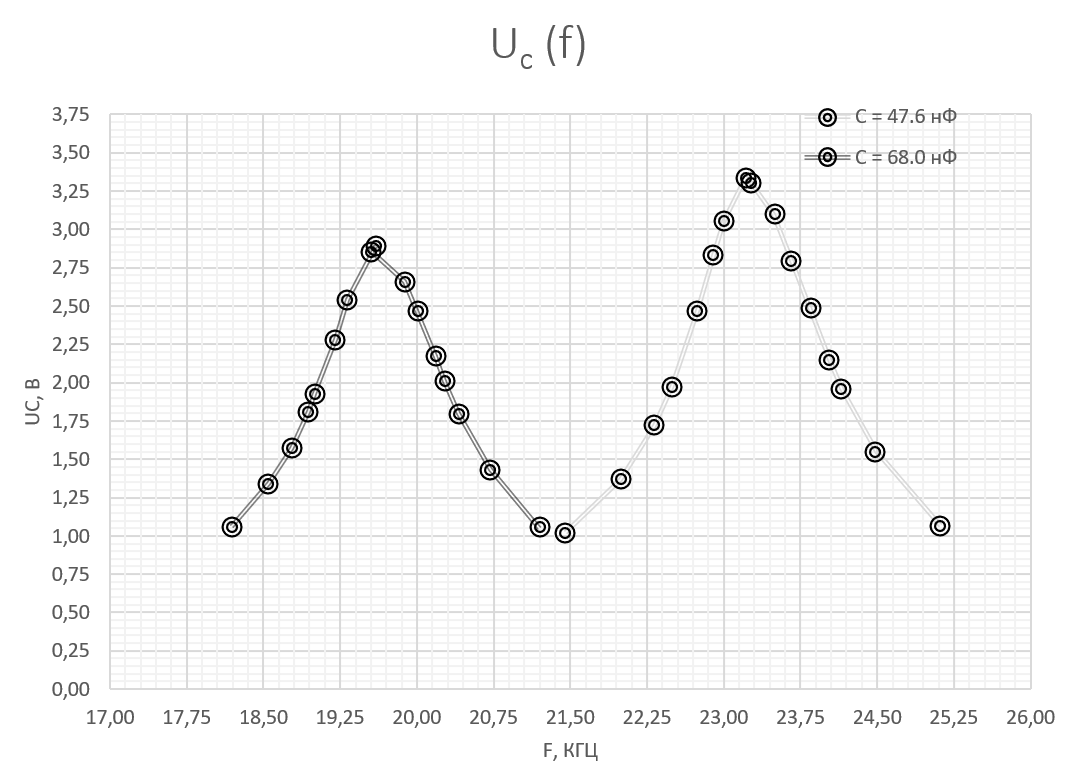
\includegraphics[width=0.85\textwidth]{3.2.2_5.png}\\
\textbf{Рис. 5.} Графики зависимости напряжения на конденсаторе от частоты (АЧХ) для двух контуров \\
\end{center}

\hfill \break По тем же данным построим также графики в безразмерных координатах: $x = f/f_{0n}$, $y = U_{C}(x)/U_{C}(1)$, где $f_{0n}$ $-$ резонансная частота для соответствующего контура:

\begin{center}
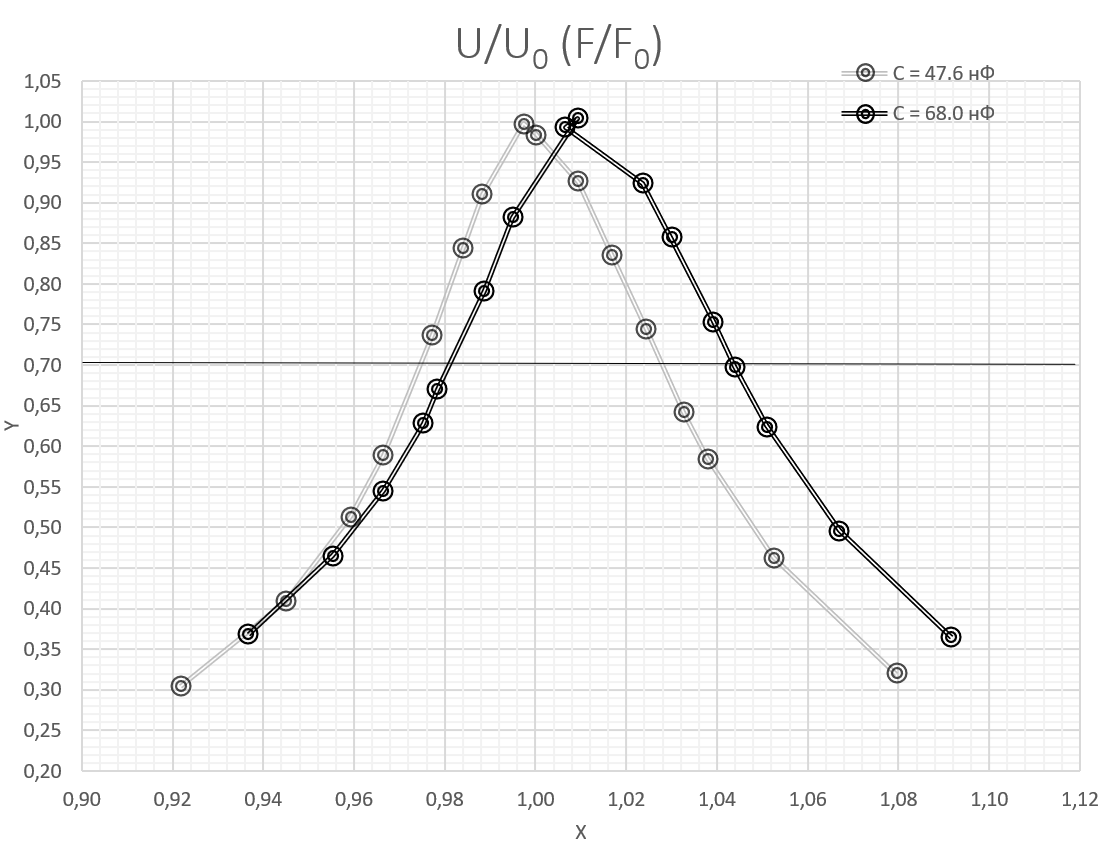
\includegraphics[width=0.85\textwidth]{3.2.2_6.png}\\
\textbf{Рис. 6.} Графики АЧХ в безразмерных координатах, где $x = f/f_{0n}$, $y = U_{C}(x)/U_{C}(1)$\\
\end{center}

\hfill \break  Из графиков 5 и 6 хорошо видно, что резонансная частота и добротность для $C_{3} = 47.6$ нФ выше. По ширине резонансных кривых (рис. 6) на уровне 0.707 определим добротности контуров как обратное к разности частот на этом уровне: 

$$
Q_{C_{3}} = 20.6 \pm 0.1;
$$

$$
Q_{C{_5}} = 17.2 \pm 0.1.
$$

\subsection{Фазово-частотные характеристики}
\hfill \break Для тех же двух контуров получим фазово-частотные характеристики $\varphi_{C}(f)$ при том же значении напряжения $E$. Результаты измерений занесем в таблицу 2:

\begin{center}
	\begin{tabular}{ccc||c|c|c|}
		\hline
		\multicolumn{3}{|c||}{$C_3 = 47.6 $ нФ} & \multicolumn{3}{c|}{$C_5 = 68.0$ нФ} \\ \hline
		\multicolumn{1}{|c|}{$n$} & \multicolumn{1}{c|}{$f$, кГц} & $-\varphi/ \pi$ & $n$ & $f$, кГц & $-\varphi/ \pi$ \\ \hline
		\multicolumn{1}{|c|}{1} & \multicolumn{1}{c|}{23.21} & 0.46 & 1 & 19.65 & 0.48 \\ \hline
		\multicolumn{1}{|c|}{2} & \multicolumn{1}{c|}{23.47} & 0.61 & 2 & 19.27 & 0.32 \\ \hline
		\multicolumn{1}{|c|}{3} & \multicolumn{1}{c|}{23.57} & 0.64 & 3 & 19.13 & 0.24 \\ \hline
		\multicolumn{1}{|c|}{4} & \multicolumn{1}{c|}{23.69} & 0.69 & 4 & 18.91 & 0.20 \\ \hline
		\multicolumn{1}{|c|}{5} & \multicolumn{1}{c|}{23.93} & 0.75 & 5 & 18.76 & 0.18 \\ \hline
		\multicolumn{1}{|c|}{6} & \multicolumn{1}{c|}{24.26} & 0.80 & 6 & 18.56 & 0.13 \\ \hline
		\multicolumn{1}{|c|}{7} & \multicolumn{1}{c|}{24.56} & 0.83 & 7 & 18.27 & 0.11 \\ \hline
		\multicolumn{1}{|c|}{8} & \multicolumn{1}{c|}{25.11} & 0.88 & 8 & 18.03 & 0.09 \\ \hline
		\multicolumn{1}{|c|}{9} & \multicolumn{1}{c|}{23.20} & 0.46 & 9 & 19.61 & 0.49 \\ \hline
		\multicolumn{1}{|c|}{10} & \multicolumn{1}{c|}{22.95} & 0.34 & 10 & 19.86 & 0.60 \\ \hline
		\multicolumn{1}{|c|}{11} & \multicolumn{1}{c|}{22.77} & 0.27 & 11 & 19.98 & 0.65 \\ \hline
		\multicolumn{1}{|c|}{12} & \multicolumn{1}{c|}{22.67} & 0.23 & 12 & 20.24 & 0.74 \\ \hline
		\multicolumn{1}{|c|}{13} & \multicolumn{1}{c|}{22.51} & 0.18 & 13 & 20.43 & 0.76 \\ \hline
		\multicolumn{1}{|c|}{14} & \multicolumn{1}{c|}{22.20} & 0.14 & 14 & 20.68 & 0.82 \\ \hline
		\multicolumn{1}{|c|}{15} & \multicolumn{1}{c|}{21.71} & 0.10 & 15 & 20.84 & 0.83 \\ \hline
		\multicolumn{1}{|c|}{16} & \multicolumn{1}{c|}{21.35} & 0.08 & 16 & 21.15 & 0.86 \\ \hline
	\end{tabular}\\
\hfill \break \textbf {Таблица 2.} Результаты измерений для ФЧХ \\
\end{center}

\hfill \break На основе данных из таблицы 2 построим на одном графике фазово-частотные характеристики в безразмерных координатах: $x = f/f_{0n}$, $y = -\varphi/\pi$:

\begin{center}
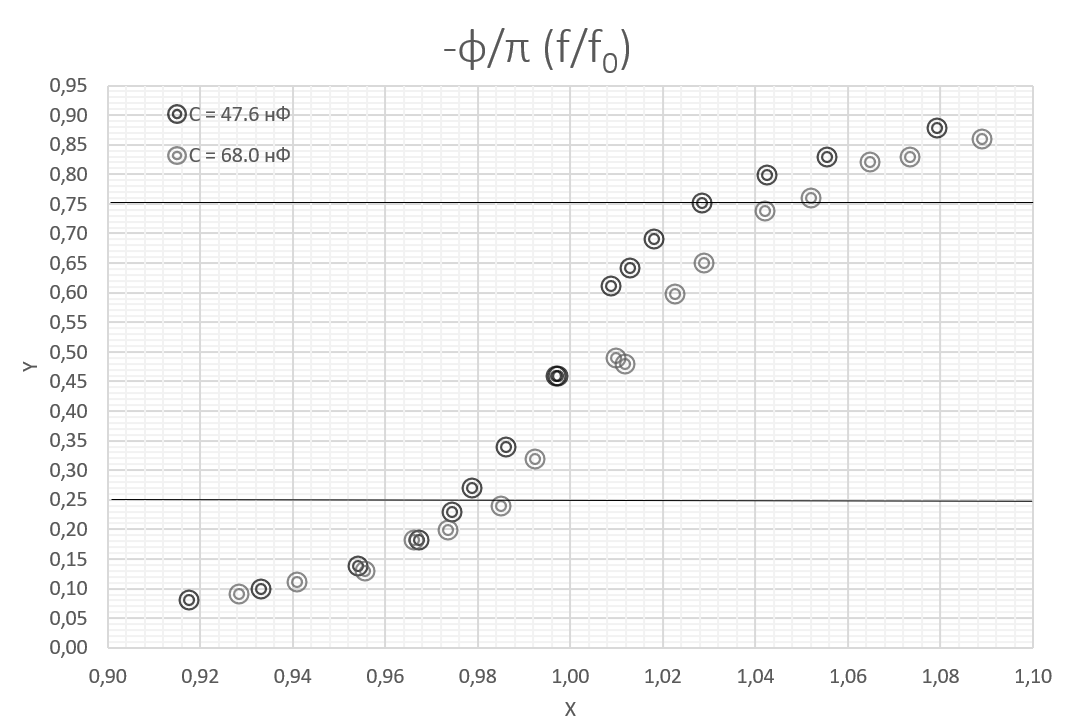
\includegraphics[width=0.85\textwidth]{3.2.2_7.png}\\
\textbf{Рис. 7.} Графики ФЧХ в безразмерных координатах, где $x = f/f_{0n}$, $y = -\varphi/\pi$\\
\end{center}

\hfill \break По полученным характеристикам (рис. 7) определим добротности контуров. По расстоянию между точками по оси $x$, в которых $y$ меняется от $1/4$ до $3/4$, равному $1/Q$, определим $Q$:

$$
Q_{C_{3}} = 20 \pm 1;
$$

$$
Q_{C_{5}} = 16 \pm 1.
$$

\hfill \break Как видно, полученные значения добротности неплохо согласуются с определенными при помощи АЧХ.

\subsection{Характеристики контура}
\hfill \break При все том же значении $E = 175.5$ мВ для контуров с семью различными емкостями $C_{n}$ измерим резонансные частоты $f_{0n}$ и напряжения $U_{C}(f_{0n})$. По результатам измерений для каждого контура определим значение индуктивности катушки $L$, добротность $Q$, характеристическое сопротивление $\rho$, суммарное сопротивление контура $R_{\Sigma}$, значение ЭПС $R_{S\text{max}}$, омическое сопротивление катушки $R_{L}$ и ток $I$. Результаты измерений и вычислений занесем в таблицу 3.

\hfill \break Зная резонансную частоту, можно найти индуктивность катушки по формуле:

$$
L = \frac{1}{4\pi^2Cf_{0}^2},
$$

\hfill \break а погрешность можно определить как

$$
\sigma_{L} = L\sqrt{\left( \frac{\sigma_{C}}{C} \right)^2 + 4\left( \frac{\sigma_{f_{0}}}{f_{0}} \right)^2}.
$$

\hfill \break Характеристическое сопротивление контура ищется как

$$
\rho = \sqrt{\frac{L}{C}},
$$

\hfill \break причем погрешность

$$
\sigma_{\rho} = \rho\sqrt{\left(\frac{\sigma_{L}}{2L} \right)^2 + \left(\frac{\sigma_{C}}{2C}\right)^2}.
$$

\hfill \break Зная суммарное активное сопротивление и $R_{S} = 10^{-3}\rho$, можно найти активное сопротивление катушки $R_{L}$. Для определения добротности контура применяется формула $U_{C}(f_{0}) = QE$. При этом $R_{\Sigma} = \frac{1}{f_{0}CQ}$. Все погрешности также занесены в таблицу 3.

\begin{center}
	\begin{tabular}{|c|c|c|c|c|c|c|c|c|c|c|c|}
		\hline
		$n$ & $C_n$, нФ & \begin{tabular}[c]{@{}c@{}}$f_{0n}$, \\ кГц\end{tabular} & $U_C$, В & $E$, мВ & \begin{tabular}[c]{@{}c@{}}$L$, \\ мкГн\end{tabular} & $Q$ & \begin{tabular}[c]{@{}c@{}}$\rho$, \\ Ом\end{tabular} & \begin{tabular}[c]{@{}c@{}}$R_{\sum}$, \\ Ом\end{tabular} & \begin{tabular}[c]{@{}c@{}}$R_{S_{\max}}$,\\ Ом\end{tabular} & $R_L$, Ом & $I$, мА \\ \hline
		1 & 24.8 & 32.20 & 4.38 & 175.5 & 986.1 & 25.0 & 199.4 & 7.99 & 0.20 & 4.34 & 21.97 \\ \hline
		2 & 33.2 & 27.78 & 3.88 & 175.5 & 989.6 & 22.1 & 172.7 & 7.81 & 0.17 & 4.19 & 22.47 \\ \hline
		3 & 47.6 & 23.27 & 3.35 & 175.5 & 983.7 & 19.1 & 143.8 & 7.53 & 0.14 & 3.94 & 23.30 \\ \hline
		4 & 57.5 & 21.17 & 3.10 & 175.5 & 983.9 & 17.7 & 130.8 & 7.41 & 0.13 & 3.82 & 23.70 \\ \hline
		5 & 68.0 & 19.42 & 2.88 & 175.5 & 988.7 & 16.4 & 120.6 & 7.35 & 0.12 & 3.78 & 23.88 \\ \hline
		6 & 81.6 & 17.73 & 2.90 & 175.5 & 988.5 & 16.5 & 110.1 & 6.66 & 0.11 & 3.63 & 26.35 \\ \hline
		7 & 102.8 & 15.82 & 2.42& 175.5 & 985.5 & 13.8 & 97.9  & 7.10 & 0.10 & 3.55 & 24.72 \\ \hline
		\multicolumn{5}{|c|}{Среднее значение} & 986.6 & 18.7 & 139.3 & 7.41 & 0.14 & 3.89 & 23.77 \\ \hline
		\multicolumn{5}{|c|}{Коэффициент Стьюдента} & 2.2 & \multicolumn{4}{c|}{--} & 2.26 & -- \\ \hline
        \multicolumn{5}{|c|}{Среднеквадратичная погрешность} & 0.1 & \multicolumn{4}{c|}{--} & 0.02 & -- \\ \hline
        \multicolumn{5}{|c|}{Случайная погрешность} & 0.3 & \multicolumn{4}{c|}{--} & 0.10 & -- \\ \hline
	\end{tabular}\\
 \hfill \break \textbf {Таблица 3.} Характеристики контуров \\
\end{center}

\hfill \break Таким образом, мы определили добротности контуров с $C_{3}$ и $C_{5}$ тремя разными способами: по АЧХ, ФЧХ и теоретически. Сравним полученные значения:

\begin{center}
    \begin{tabular}{|c|c|c|c|}
        \hline
        $ $ & $Q$, АЧХ & $Q$, ФЧХ & $Q$, теория \\\hline
        $C_{3} = 47.6$ нФ & $20.6 \pm 0.1$ & $20 \pm 1$ & $19.1$ \\\hline
        $C_{5} = 68.0$ нФ & $17.1 \pm 0.1$ & $16 \pm 1$ & $16.4$ \\\hline
    \end{tabular}\\
 \hfill \break \textbf {Таблица 4.} Добротности контуров, вычисленные тремя способами \\
\end{center}

\hfill \break По данным таблицы 3 построим график зависимости сопротивления катушки индуктивности от резонансной частоты $R_{L} (f_{0n})$:

\begin{center}
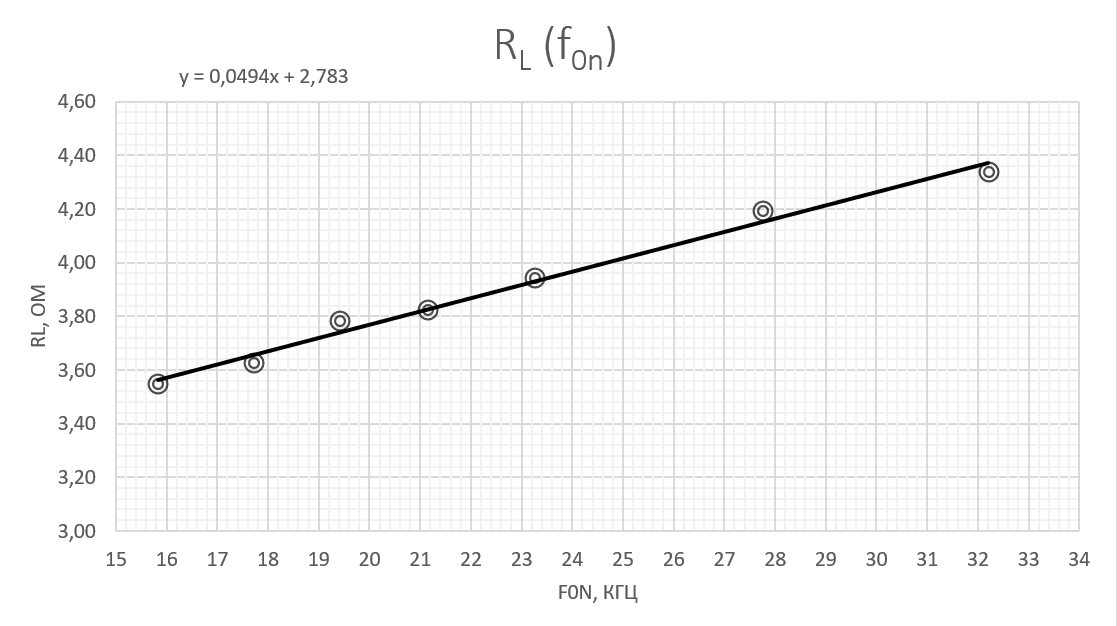
\includegraphics[width=0.90\textwidth]{3.2.2_8.png}\\
\textbf{Рис. 8.} График зависимости сопротивления катушки индуктивности от резонансной частоты\\
\end{center}

\hfill \break Уравнение полученной зависимости указано на графике (рис. 8). Видим, что с увеличением частоты резонанса (то есть с увеличением емкости в цепи) растет и сопротивление потерь катушки. Можно предположить, что изменения связаны с потерями на перемагничивание сердечника катушки.  

\subsection{Векторная диаграмма}
\hfill \break Построим векторную диаграмму напряжений для контура с наименьшей добротностью в резонансном состоянии, ось абсцисс направим по вектору $\textbf{E}$, а масштаб оси сделаем в 2 раза более крупным, чем оси ординат. Так как, по закону Кирхгофа, $E = U_{R} + U_{C} + U_{L}$, на графике вектор $\textbf{E}$ должен быть равен сумме остальных векторов напряжений. 

\begin{center}
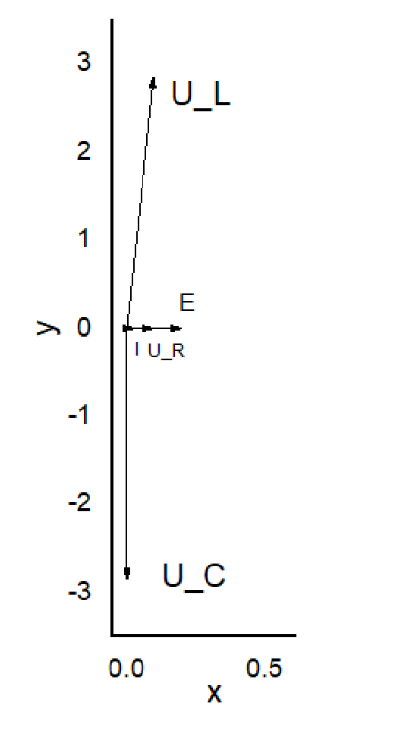
\includegraphics[width=0.25\textwidth]{3.2.2_9.png}\\
\textbf{Рис. 9.} Векторная диаграмма \\
\end{center}

\section{Вывод}
\hfill \break Было проведено исследование резонанса напряжений в последовательном колебательном контуре, по результатам которого были определены некоторые его характеристики: индуктивность, сопротивление катушки индуктивности, характеристическое сопротивление. Также тремя разными способами были рассчитаны добротности двух контуров.

\end{document}
